\section{Реализация алгоритма SCC}

Алгоритм SCC был реализован в~виде пакета процедур \verb|StrongCyclicityChecking| для~Мэйпл.
В~этом разделе мы рассмотрим программную реализацию данного проекта.


\subsection{Система компьютерной алгебры Мэйпл}

Мэйпл является системой для~работы с~компьютерной алгеброй~\cite{litMapleHelp}.
Мэйпл предоставляет колоссальное количество возможностей для~математических вычислений, визуализации данных и моделирования.
Когда пользователь запускает систему и создает новый документ,
на~экране появляется рабочая область, в~который он может вводить формулы, выражения и т.д.
Это выглядит следующим образом:

\begin{center}
    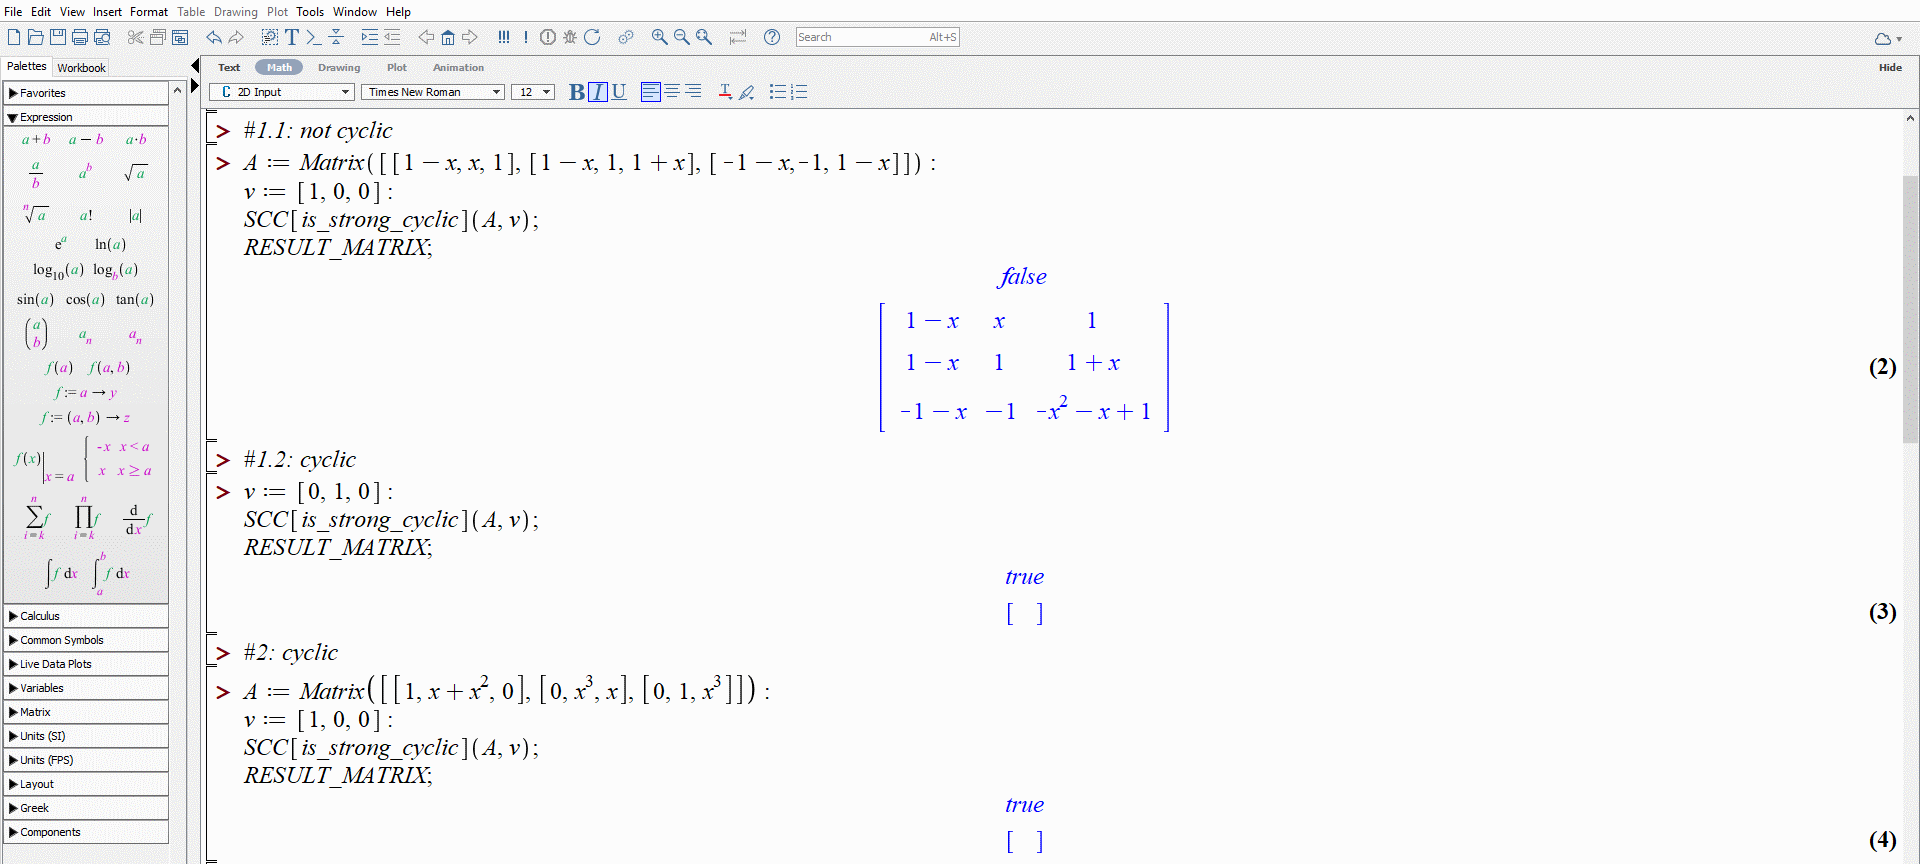
\includegraphics[scale=0.3]{pictures/maple_workarea.png}

    \small
    Рис. 7.1. Рабочая область в Мэйпл
\end{center}

Рабочая область состоит из~последовательных ячеек, содержащих обычный текст или математические выражения.
По команде пользователя все содержимое ячейки может быть выполнено, при~этом результаты вычисления появятся под~ячейкой.
Эти результаты могут быть использованы в~дальнейших расчетах.

Мэйпл предоставляет свой собственный язык программирования \cite{litMapleGuide2011, litMapleGuide2021},
который может быть использован для~реализации своих собственных процедур и структур данных.
Присутствуют все обычные элементы императивной парадигмы программирования:
циклы, присваивания, переменные, условные выражения, списки и пр.
Реализованные процедуры могут быть объединены в~\emph{пакет процедур}
для~дальнейшего использования в~Мэйпл.

\newpage

\subsection{Архитектура пакета}

Для удобства содержимое пакета было разбито на~4~файла, каждый из~которых выполняет свою функцию:

\begin{itemize}
    \item
        \verb|polynom.mm| "--- содержит базовые процедуры для~работы с~полиномами:
        \begin{itemize}
            \item
                \verb|max_degree| "--- определение максимальной степени~$x$ в~выражении;
            \item
                \verb|prolong| "--- построение продолжения многочлена указанным слагаемым.
        \end{itemize}
    \item
        \verb|cyclic.mm| "--- содержит базовые процедуры для~работы с~циклическими векторами:
        \begin{itemize}
            \item
                \verb|CV_dv| "--- построение матрицы производных вектора в~силу системы.
        \end{itemize}
    \item
        \verb|strong_cyclic.mm| "--- содержит реализацию основной процедуры \verb|is_strong_cyclic| проверки того,
        является~ли вектор сильно циклическим;
    \item
        \verb|strong_cyclicity_checking.mpl| "--- главный файл пакета, объединяющий все в~единое целое.
\end{itemize}

Далее приведено более подробное описание реализованных процедур.
Исходный код данных процедур приведен в \emph{Приложении А}.

\begin{itemize}
    \item
        Процедура для~определения степени многочлена:
        
        \verb|max_degree := proc(p)|

        Единственный ее параметр \verb|p| "--- выражение, имеющее вид многочлена от~$x$,
        которое может дополнительно содержать слагаемое вида~$O(x^t)$.
        Возвращает степень многочлена, которая затем будет использоваться при~построении продолжения данного многочлена.

    \item
        Процедура для построения продолжения многочлена:
        
        \verb|prolong := proc(p, coef, degree)|

        Принимает 3 параметра:
        \begin{itemize}
            \item
                \verb|q| "--- многочлен от~переменной~$x$;
            \item
                \verb|coef| "--- символьный или числовой коэффициент;
            \item
                \verb|degree| "--- степень, которой необходимо продолжить многочлен.
        \end{itemize}

        Процедура возвращает новый многочлен, являющийся продолжением многочлена~\verb|q(x)|.
        Продолжение получается добавлением к~многочлену нового слагаемого~\verb|coef| $\cdot x^{degree}$.

    \item
        Процедура для~построения матрицы производных в~силу системы:
        
        \verb|CV_dv := proc(A, v, m)|
        
        \newpage
        Принимает 2 или 3 параметра:
        \begin{itemize}
            \item
                \verb|A| "--- квадратная матрица с коэффициентами, являющимися полиномами от~независимой переменной~$x$,
                элементы также могут содержать слагаемые вида~$O(x^t)$;
            \item
                \verb|v| "--- вектор с~коэффициентами, являющимися полиномами от~независимой переменной~$x$;
            \item
                \verb|m| "--- количество столбцов результирующей матрицы, которое нужно вычислить
                (значение по~умолчанию: размер матрицы~\verb|A|).
        \end{itemize}

        Данная процедура возвращает матрицу,
        столбцами которой являются $v$, $\diffVector$, $\diffVector[2]$, $\cdots$, $\diffVector[m-1]$.
        При $m=n$ эта матрица будет являться матрицей производных в~силу системы для~матрицы~\verb|A| и вектора~\verb|v|,
        которая может использоваться для~определения~того, является~ли вектор~\verb|v| циклическим.
\end{itemize}

Сам алгоритм проверки сильной цикличности вектора был реализован в~виде двух процедур:
\begin{itemize}
    \item
        \verb|is_strong_cyclic| "--- процедура, которую непосредственно вызывает пользователь;
        вызывает рекурсивную процедуру с~нужными параметрами;
    \item
        \verb|is_strong_cyclic_process| "--- рекурсивная процедура, выполняющая основные вычисления.
\end{itemize}

Более подробно про эти процедуры:
\begin{itemize}
    \item
        \verb|is_strong_cyclic := proc(A, v, max_recursion_depth)|

        Принимает 2 или 3 параметра:
        \begin{itemize}
            \item
                \verb|A| "--- квадратная матрица с коэффициентами, являющимися полиномами от~независимой переменной~$x$,
                элементы также могут содержать слагаемые вида~$O(x^t)$;
            \item
                \verb|v| "--- вектор с~коэффициентами, являющимися полиномами от~независимой переменной~$x$;
             \item
                \verb|max_recursion_depth| "--- целое число,
                ограничивающее допустимую глубину рекурсии при~построении опровергающего продолжения.
                Если не~задано, будет использовано значение по~умолчанию (см.~ниже).
        \end{itemize}

        Использование слагаемых вида~$O(x^t)$ в матрице \verb|A| позволяет указывать процедуре~то, какие степени многочленов
        представлены в~коэффициентах.
        Например, выражение $x + 4x^2 + O(x^5)$ следует интерпретировать как~многочлен 4-й степени,
        у~которого коэффициенты перед~3-й и 4-й степенью равны нулю.

        \newpage
        Возвращает одно~из~трех логических значений:
        \begin{itemize}
            \item
                \verb|false| "--- вектор не~является сильно циклическим;
                в переменной \verb|RESULT_MATRIX| (см. ниже) будет содержаться построенное опровергающее продолжение.
            \item
                \verb|true| "--- вектор является сильно циклическим.
             \item
                \verb|fail| "--- не~удалось получить ответ (уперлись в~максимально допустимую глубину рекурсии
                при~построении продолжения).
        \end{itemize}

    \item
        \verb|is_strong_cyclic_process := proc(A, v, steps_left, degree_matrix)|

        Принимает 4 параметра:
        \begin{itemize}
            \item
                \verb|A| "--- квадратная матрица с~коэффициентами, являющимися полиномами от~независимой переменной~$x$,
                элементы также могут содержать слагаемые вида~$O(x^t)$
            \item
                \verb|v| "--- вектор с~коэффициентами, являющимися полиномами от~независимой переменной~$x$
            \item
                \verb|steps_left| "--- целое число,
                указывающее максимально допустимую глубину рекурсии для~данного этапа.
            \item
                \verb|degree_matrix| "--- квадратная матрица того~же размера, что и~\verb|A|,
                содержит целые числа "--- степени многочленов в~соответствующих элементах матрицы~\verb|A|.
        \end{itemize}
\end{itemize}


Пользователь имеет доступ к~нескольким глобальным переменным, которые могут регулировать работу алгоритма:
\begin{itemize}
    \item
        \verb|MAX_RECURSION_DEPTH| "--- целое число, являющееся значением по~умолчанию для~максимально допустимой глубины рекурсии.
        По умолчанию равно~10.
    \item
        \verb|VERBOSE| "--- булевый флаг, при установке в~\verb|true| процедура будет подробно показывать процесс вычислений.
        По умолчанию равно~\verb|false|.
    \item
        \verb|RESULT_MATRIX| "--- в~эту переменную будет записана матрица, являющаяся опровергающим продолжением,
        в~случае, когда удалось построить опровергающее продолжение.
\end{itemize}


\newpage
\subsection{Использование пакета StrongCyclicityChecking}

Исходный код пакета доступен по адресу\\
\url{https://github.com/KingAArtur/strong-cyclicity-checking}.

\medskip
На рис.~7.2 и 7.3 приведены примеры использования процедуры \verb|is_strong_cyclic|.


\begin{center}
    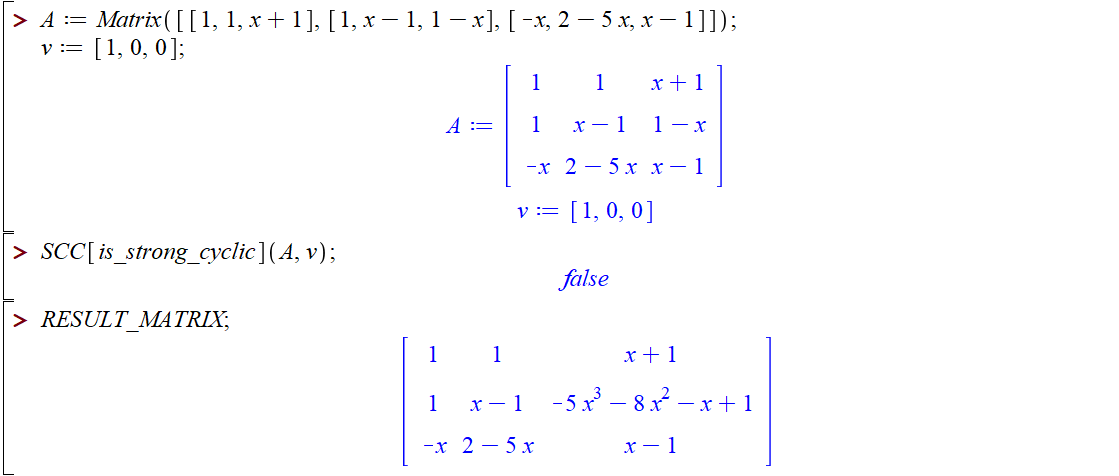
\includegraphics[scale=0.6]{pictures/maple_example4.png}

    \small
    Рис. 7.2. Пример работы процедуры для~не~сильно циклического вектора
\end{center}


\begin{center}
    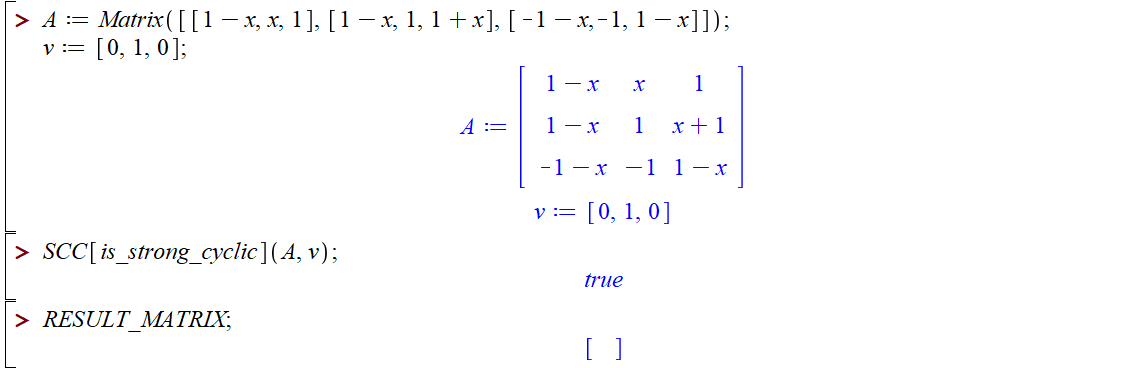
\includegraphics[scale=0.6]{pictures/maple_example1.png}

    \small
    Рис. 7.3. Пример работы процедуры для~сильно циклического вектора
\end{center}

Больше примеров можно найти по адресу\\
\url{https://github.com/KingAArtur/strong-cyclicity-checking}.